\RequirePackage[OT1]{fontenc}
\documentclass[conference]{IEEEtran}
% \hypersetup{draft}

\usepackage{multirow}
\usepackage{tabulary}
\usepackage{tabularx}
\usepackage{pdfpages}
\usepackage{amsmath,amssymb,stmaryrd}   
\usepackage{anyfontsize}
\usepackage{multicol}
\usepackage{booktabs}
\usepackage[lined,linesnumbered,commentsnumbered,ruled]{algorithm2e}
% \usepackage{algorithm}
% \usepackage{algorithmic}
\usepackage{algpseudocode}
\usepackage{listings}
\usepackage{wrapfig}
% \usepackage{placeins}
\usepackage{float}
% \usepackage{algorithm2e}
\usepackage{longtable}
\usepackage{etoolbox}
\usepackage[utf8]{inputenc}
\usepackage[T1]{fontenc}
\usepackage{adjustbox}
\usepackage{siunitx}
\usepackage{url}
\usepackage{lscape,lipsum}
\usepackage{everypage}
\usepackage{eurosym}
\usepackage{hyperref}

\usepackage[backend=biber, style=numeric]{biblatex}
	\addbibresource{/home/aghiles/Aghiles/Redaction/lib/iot.bib}%
	\addbibresource{/home/aghiles/Aghiles/Redaction/lib/iotbis.bib}%

\def\Mark#1{\textsuperscript#1}

\usepackage{graphicx}
	\graphicspath{ {Figures/} }
\usepackage{subcaption}
	\captionsetup{justification=centering}
	\captionsetup[table]{skip=10pt}
%	\captionsetup{labelfont=it,textfont={bf,it},justification=centering}
	\renewcommand{\thesubfigure}{\alph{subfigure}}
	\renewcommand{\thefigure}{\arabic{figure}}

\newcommand{\Figure}[4]{
	\begin{figure}[#1]
	\centering
	\includegraphics[width=#2\columnwidth]{#3}
	\caption{#4.}\label{fig:#3}
	\end{figure}
}

\newcommand{\FigureH}[8]{
%	\medskip
	\begin{figure}
		\centering
		\begin{subfigure}[#1]{#2\columnwidth}
			\centering
			\includegraphics[width=\columnwidth]{#3}
			\caption{#4.}\label{fig:#3}
		\end{subfigure}
		~ % \quad, \qquad, \hfill
		\begin{subfigure}[#1]{#2\columnwidth}
			\centering
			\includegraphics[width=\columnwidth]{#5}
			\caption{#6.}\label{fig:#5}
		\end{subfigure}
		
		\caption{#8.}\label{fig:#7}
	\end{figure}
%	\medskip
}



\def\ac#1{{#1}}

\author{
	Rafik Zitouni\Mark{2}, Jerimie ...\Mark{2}, Aghiles Djoudi\Mark{1}\Mark{2} and Laurent George\Mark{1}	\bigskip\\
	\Mark{1}LIGM/ESIEE Paris, 5 boulevard Descartes, Champs-sur-Marne, France\\
	\Mark{2}SIC/ECE Paris, 37 Quai de Grenelle, 75015 Paris, France\\
	Email:   \{aghiles.djoudi, nawel.zangar, laurent.george\}@esiee.fr, rafik.zitouni@ece.fr
}

% \author{
% 	\IEEEauthorblockN{
% 		Aghiles Djoudi\Mark{1}\Mark{2}, Rafik Zitouni\Mark{2}, Nawel Zangar\Mark{1} and Laurent George\Mark{1}
% 	}
% 	\IEEEauthorblockA{
% 		\Mark{1}LIGM/ESIEE Paris, 5 boulevard Descartes, Champs-sur-Marne, France\\
% 		\Mark{2}SIC/ECE Paris, 37 Quai de Grenelle, 75015 Paris, France\\
% 		Email:   \{aghiles.djoudi, nawel.zangar, laurent.george\}@esiee.fr, rafik.zitouni@ece.fr
% 	}
% }


\begin{document}

%\setcounter{page}{1}
\title{Genetic Algorithm For LoRa Transmission Parameter Selection}
\maketitle

	\begin{abstract}

% Problem
Most traffic light's control systems in smart cities are wired and have a semi-static behavior.
They are time-based, with pre-configured pattern and expensive cameras.
% Existing solutions
Although traffic lights can communicate wirelessly with incoming vehicles,
	they are less adapted to an urban environment.
If we consider light signs as an Internet of Things (IoT) network,
	one issue is to model thoroughly the change of signs' states and the Quality of Service (QoS) of this network.
In this paper,
	we propose a new architecture of Urban Traffic Light Control based on an IoT network (IoT-UTLC).
The objective is to interconnect both roads' infrastructures and traffic lights through an IoT platform.
We designed our IoT-UTLC by selecting motes and protocols of wireless sensor network (WSN).
Message Queuing Telemetry Transport (MQTT) protocol has been integrated to manage QoS.
It enables lights to adapt remotely to any situation and smoothly interrupt traffic light's classic cycles.
Our experimental results show that the MQTT protocol is efficient when the packets rate exceeds 35\% of traffic flow,
	it reduces traffic delay up to 0.05s at 90\% of congestion.
After verification and validation of our solution using a UPPAAL model checker,
	our system has been prototyped.
Motes' functions have been implemented on Contiki OS and connected through a 6LoWPAN/IEEE 802.15.4 network.
Time-stamping messages have been performed throughout the system to evaluate the MQTT protocol with different QoS levels.
In our experiments,
	we measured the Round-trip delay time (RTT) of messages exchanged between the WSN and IoT Cloud.
The results show that MQTT decreases the RTT when the Cumulative Distributed Function (CDF) of generated messages exceeds 35\%.

\end{abstract}
	\section{Introduction} \label{sec:Introduction}




\subsection{Problem Statement}

\subsection{Background}

\subsection{Purpose (Goal)}

\subsection{Limitations}

\subsection{Method}


% The structure 
This paper is organized as follows.
Section \ref{sec:Related work} elucidates summary of related works.
% Section \ref{sec:Background} provide the required background.
In section \ref{sec:Approach}, we propose our ... to ....
Section \ref{sec:Experimentation} evaluates the performance of our ... in terms of packet delivery ratio,
	throughput,
	and power consumption.
% Our findings are presented in section \ref{sec:Results}.
Section \ref{sec:Conclusion} concludes the article and gives some ideas for future work.


% Needs by statistics: Context Current needs


% Problematic Current bad state of the research


%Challenges
The difficulty to build such system is 


%Contribution 
In this work we 

% The structure 
The article is organized as follows.
Section \ref{sec:Related work} elucidates summary of related works,
In section \ref{sec:Approach}, we propose our ... to ....
Section \ref{sec:Experimentation} evaluate the performance of our ... in terms of packet delivery ratio,
	throughput,
	and power consumption.
Section \ref{sec:Conclusions} concludes the article and gives some ideas for future work.





	\section{Related work} \label{Sec:Related_Works}

Petri nets (PNs) are widely used for traffic light modelling and control \cite{huang_modular_2014}.
In  \cite{difebbraro_trafficresponsive_2006},
	deterministic-timed Petri Nets have been used to describe signalized intersections.
Undesirable deadlock states might appear when the nets are tested for some use cases.
The authors in \cite{febbraro_using_2009} have modified PNs models including  stochastic-time for one single signalized intersection.
Dotoli and Fanti \cite{dotoli_urban_2004} have built a colored timed PN with a deterministic modular framework,
	in which parts of the system,
	and even parts of the subsystems,
	can be specified and analyzed separately.
Examples using modularity are given in Soares and Vrancken \cite{dossantossoares_modular_2012},
	in which a p-timed PN is used for the control of a traffic signal in both main road and side streets.
However,
	formal characteristics of PNs (\emph{e.g.},
	deadlock and liveliness) haven’t been discussed.
Moreover,
	PNs suffer from a lack of analysis and verification tools.
To overcome these limits of PNs,
	we propose UPPAAL timed automata for design and verification of coherent state of cross road's traffic light.
UPPAAL is a timed-based modelling software with a graphical user interface.
It is the result of the research works of two universities UPPsala University in Sweden (UPP) and AALborg University in Denmark (AAL) \cite{david_uppaal_2015}.

In \cite{Web0},
	thermal cameras and on-street wired sensors detect vehicles and pedestrians in order to adapt the cycle of traffic light control systems.
However,
	such a solution can be expensive.
In addition,
	the system uses only its local view of the environment to detect the arrival of a vehicle.
Other solutions use recent technologies such as wireless sensors devices to limit the cost of thermal cameras and reduce the time needed to deploy sensors.
In \cite{tlig_decentralized_2014} and \cite{rose_internet_2015},
	the authors propose an adaptive system based on local wireless communication between lights and vehicles.
But such a solution requires a global interconnection between all road's users and infrastructure.
This problem comes from the rigid definition of technologies' standards.
Our work is not only limited to establish WSN,
	but it is scalable to interconnect heterogeneous wireless technologies through the Internet.
The obtained WSN intends to meet multiple QoS requirements of IoT applying the MQTT protocol.
In \cite{Silva2018},
	the latency of MQTT has been evaluated by calculating the average round-trip delay between two clients located in two different continents.
However,
	the evaluation has been limited to the impact of messages' size.
In our work,
	we consider the period of generated messages,
	and we calculate the RTT delays from WSN to Cloud IoT plateform.

In \cite{huang_modular_2014} \cite{difebbraro_trafficresponsive_2006} \cite{febbraro_using_2009} \cite{dossantossoares_modular_2012},
	the authors focus only on the structural analysis of their models and the transitions between colors of traffic lights.
However,
	the implementation of their models as a service in the Internet of smart cities has not been discussed.
Moreover,
	their methodology is not tested with any real traffic lights' Testbed.

	\section{Proposed Framework} \label{sec:Approach}


% A generic scheme to solve the configuration selection problem and any other similar selection problem is given in this section..
% The genetic selection scheme consists of three main steps,
% 	the first step contains a set of small parallel fuzzy logic (FL)-based subsystems,
% 	the second step is a multiple criteria decision making (MCDM) system,
% 	and the third step is a genetic algorithm (GA)-based component to assign a suitable weight for the criteria in the second component.
% The scheme decision phase can be described in more detail as follows.


% \begin{figure}
% \placetextbox{0.75}{0.8}{
% 		\tiny \mywhiteblackbox{
% 		\begin{tabular}{l} 
% 			Source program \\\hline
% 	        Ada\\
% 	        C/C++\\
% 	        Java\\ 
% 		    Perl\\
% 		    Python\\
% 		    ...
% 	    \end{tabular}
% 	}
% }
% \end{figure}


% \Figure{h}{.5}{drawing.svg}{kjkjkj rd}
	% \begin{tikzpicture}
	% 	\scriptsize
	% 	% \node[draw,align=left,dashed, text width = 0.2\linewidth] at (3,6) {Criteria c1 fuzzy based control};

	% 	\node[draw,align=left,dashed, text width = .5cm, text height = .5cm] at (3,6) {Multiple criteria decision making};
	% 	\node[draw,align=left,dashed, text width = 2cm, text height = 2cm] at (6,6) {Multiple criteria decision making};
	% 	\node[draw,align=left,dashed, text width = 2cm, text height = 2cm] at (6,3) {Genetic algorithm to determine weights of criteria (w1, ..., wn)};
	% 	\draw[->,black,thick,dashed] (0,0) -- (1,1);
	% \end{tikzpicture}

% \textbf{Definition:} stopping criteria, population size P, and mutation probability pm\\
% \textbf{Generate} randomly the initial configurations \\
% \textbf{repeat:}\\
% . . . \textbf{for} each configuration do\\
% . . . . . . Train a model \& compute configuration's fitness\\
% . . . \textbf{end}\\
% . . . \textbf{for} each reproduction 1 ... P/2 do\\
% . . . . . . \textbf{Select:} 2 configurations based on fitness\\
% . . . . . . \textbf{Crossover:} Produce 2 child configurations\\
% . . . . . . \textbf{Mutate:} child configurations with pm\\
% . . . \textbf{end}\\
% \textbf{until} stopping criterion are met\\

% \State\textbf{Definition:} stopping criteria, population size P, and mutation probability pm\\
% \State\textbf{Generate} randomly the initial configurations


\begin{algorithm}
	 \KwData{QoS constraints}
	 \KwResult{Ranked configuration list}



\SetKwFunction{FMain}{Main}
\SetKwProg{GA}{GA}{:}{end}
\GA{}{
	\Repeat{stopping criterion is met}{
		\For{each configuration}{
			Train \& compute configuration's fitness
		}
		\For{each reproduction 1 ... P/2}{
			\textbf{Select:} 2 configurations based on fitness\;
			\textbf{Crossover:} Produce 2 child configurations\;
			\textbf{Mutate:} child configurations with pm\;
		}
	}
}

% \SetKwFunction{FMain}{Main}
% \SetKwProg{FL}{FL}{:}{end}
% \FL{}{
%     \eIf{$error \geq e$}{
%         Do that as well
%     }{
%         Do otherwise
%     }
%     \While{$something \not= 0$ }{	
%         $var1 \leftarrow var2$  	
%     }

% }
% \eIf{understand}{
%   go to next section\;
%   current section becomes this one\;
% }{
%   go back to the beginning of current section\;
% }

\caption{LoRa Transmission Parameter Selection}
\end{algorithm}
\medskip

The scheme selection process can be described following these five steps:

\begin{enumerate}
	\item According to the Semtech SX1276 specification\cite{lorasemtech}, there is 6720 possible settings ($s_{1}$, ... ,$s_{6720}$) and the framework has to select the most optimal one or to rank them according to their relevance.
	\item The first step of the selection process depends on multiple criteria up to i ($c_{1}$, ... , $c_{i}$).
		Different type of criteria can be measured from different sources to cover the maximum point of views,
		as example,
		the network server requirements, the applications requirements and the devices conditions.
	\item The Fuzzy Logic (FL) based subsystem gives an initial score for each configuration that reflects its relevance.
		The different sets of scores ($d_{1}$, ... ,$d_{i}$) are sent to the \ac{MCDM} in the $5^{th}$ step.
	\item At the same time,
			the genetic algorithm (GA) \cite{alkhawlani_access_2008} assigns a suitable weight ($w_{1}$, ... ,$w_{i}$) for each initial selection decision according to the objective function that is required by the application.
			% according to the importance and sensitivities of ANS criteria to the different characteristics of a wireless heterogeneous environment.
	\item Using the initial scores coming from the $3^{rd}$ step and the weights that are assigned using the $4^{th}$ step,
			the multi criteria decision making{} \ac{MCDM} will select the most relevant settings and rank them according to their reward.
\end{enumerate}


\Figure{h}{1}{genetic}{The proposed scheme for LoRa transmission parameters selection based on \ac{GA}, \ac{FL} and \ac{MCDM}}

	\section{Prototyping} \label{sec:Experimentation}

% Intro
We have prototyped the wireless sensors and actuator's network of traffic lights and roads on a mockup \footnote{https://github.com/IoT-UTLC/Resources/wiki} of real intersection in Paris with a scale of 1:68.
Our specifications have been defined considering the low-cost and energy efficiency of the solution.
This Testbed is a proof of concept of not limited to our use case as it is scalable for other applications.
For example,
	additional sensors of fine particules could be implanted bringing correlation between traffic jam and pollution.

\begin{figure*}[!htb]
\centering
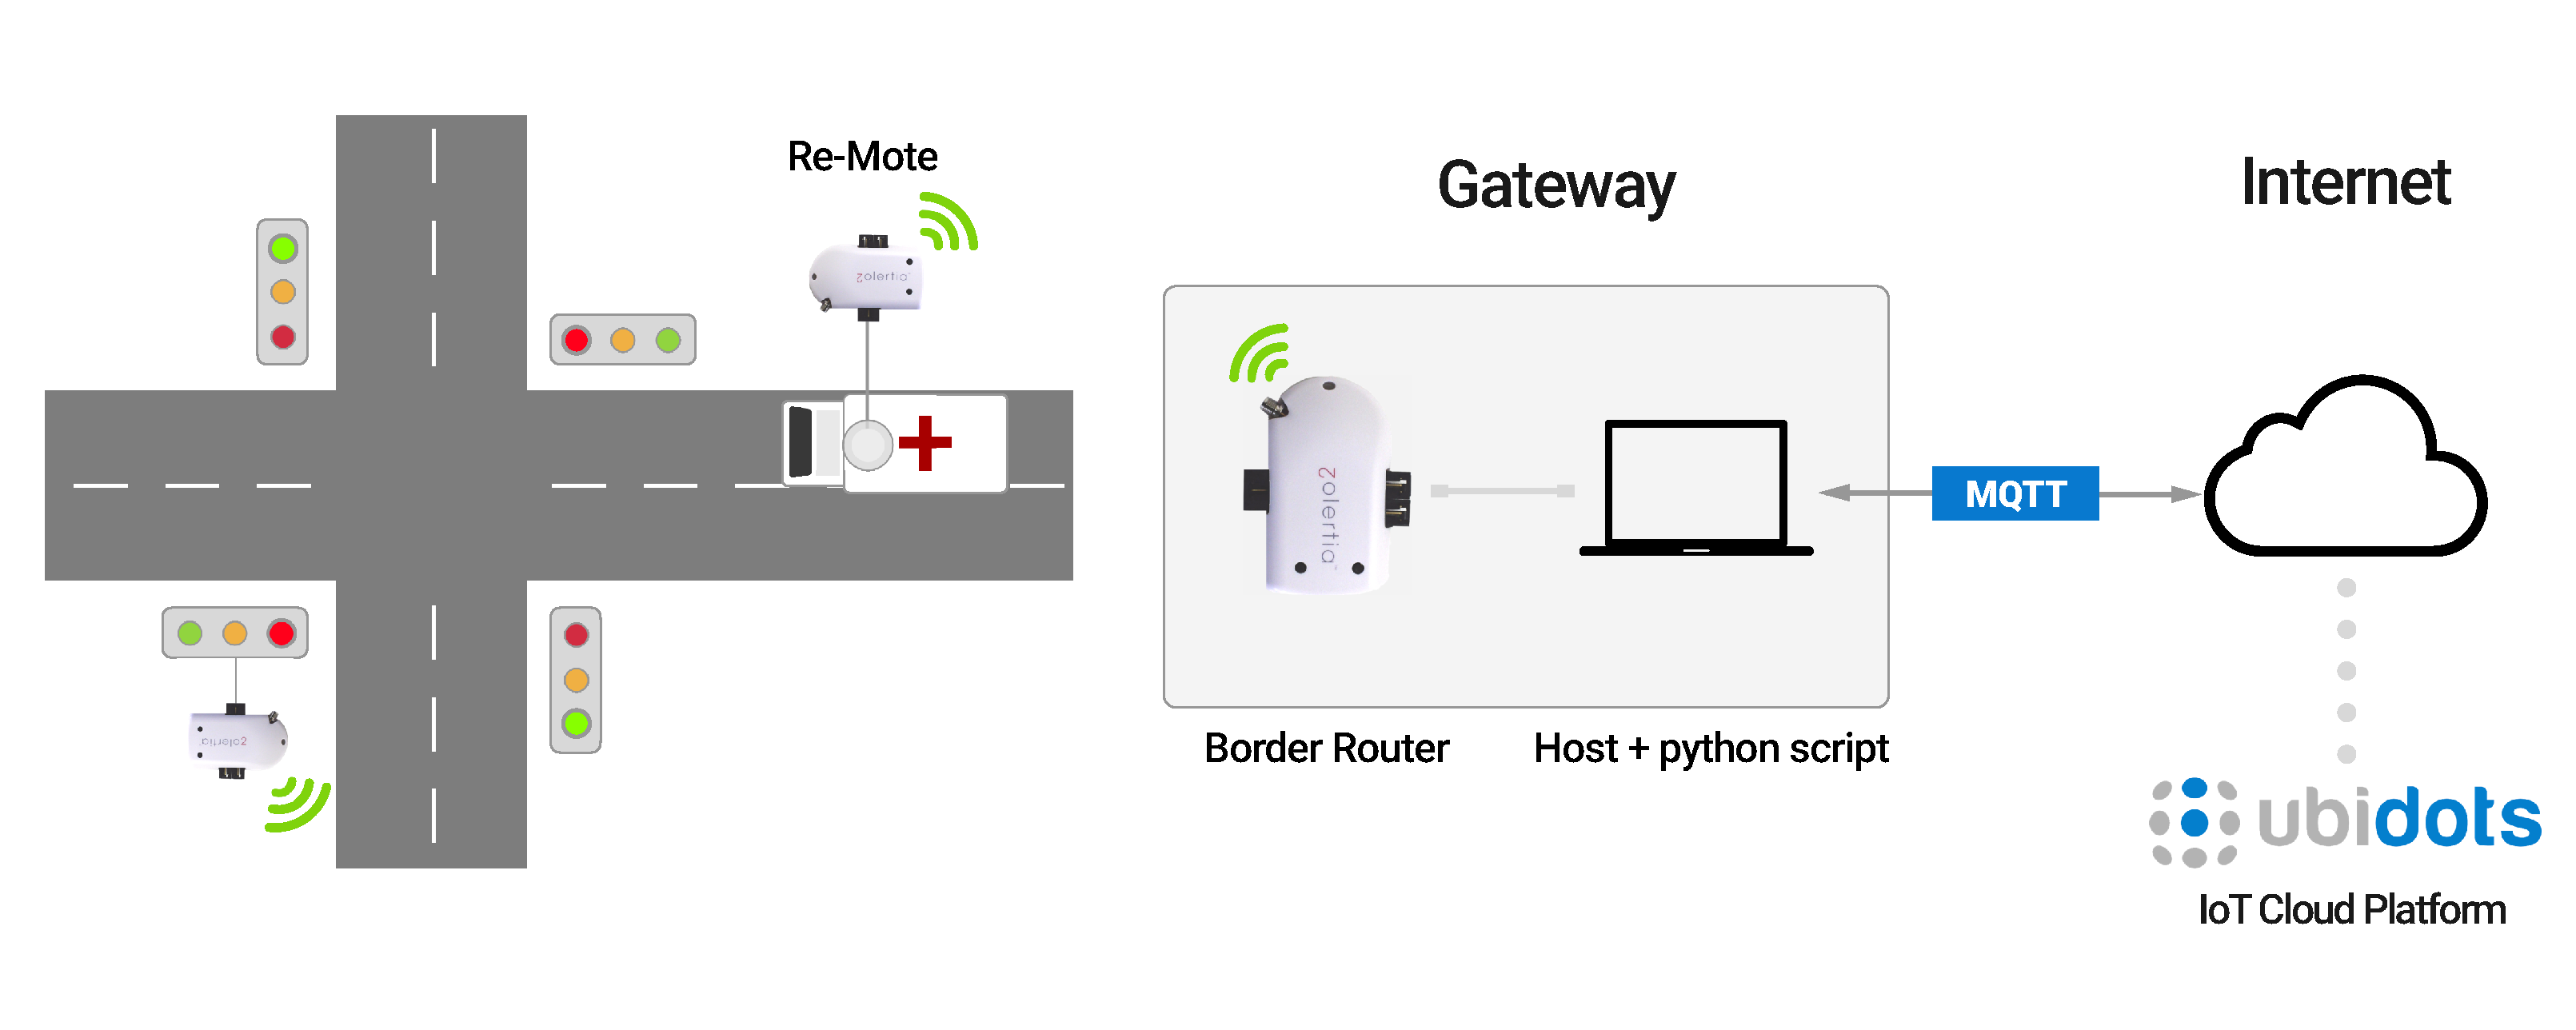
\includegraphics[width=4.5in]{Figures/ScenarioPaper.eps}
\caption{Architecture of  Iot-UTLC}
\label{fig:ScenarioPaper.eps}
\end{figure*}

Fig.
\ref{fig:ScenarioPaper.eps} shows the architecture of our IoT-UTLC with three layers.
From left to right,
	we have the WSN layer with connected traffic lights’ actuators,
	sensors and IEEE 802.15.4 transceivers.
The second part is the gateway of the WSN ensured by the BR and the Middleware \emph{i.e.} Python script launched by host computer.
The last layer is the Ubidots IoT Cloud Platform.
It is an open source solution used to collect and analyze WSN data.

\subsection{6LoWPAN, Contiki OS, Re-Mote and Border Router} \label{Sec:Contiki}

% 6LoWPAN
Our WSN is an IPv6 LowPower Wireless Personal Area Network (6LoWPAN) based on IEEE 802.15.4 stack.
It is well adapted to embedded wireless devices with energy aware constraint and for its capabilities to define a mesh topology.
Contiki Os\footnote{http://www.contiki-os.org/} has been used to implement networks' functions such as send,
	receive and data processing.
It is an embedded operating system with large open source community.
It supports Zolertia's Re-Motes \footnote{https://github.com/Zolertia/Resources/wiki/RE-Mote} and implements recent IEEE 802.15.4 standard specifications.
It also includes protocols such as RPL,
	CoAP and MQTT.
Furthermore,
	developer community is active and makes available source codes examples in order to help developing quickly new applications.

% Re-motes
Re-motes are compatible with our WSN specifications and our design model.
They are wireless devices with ultra-low power operation mode.
This choice has been motivated by long radio range of its IEEE 802.15.4 CC1200 transceiver,
	which transmits in the frequency band of 868-915 MHz.
In addition,
	each Re-Mote has analog and digital ports with a possibility to connect several analog sensors and actuators.
A Re-mote can be driven by a computer and become a sink and/or BR as well as a gateway between the 6LoWPAN network and the computer.

%\Figure{!htb}{1}{ethernetRouter.png}{Our Ethernet router}
\begin{figure}[!htb]
\centering
\includegraphics[width=2.5in]{Figures/ethernetRouter.png}
\caption{BR and sink combined on one board}
\label{fig:ethernetRouter.png}
\end{figure}

%[Explanation of how it works with the 2 radios,
To implement the previous model described in Section \ref{sec:Use Case and Model Design},
	we used six Re-motes:
	one for the BR,
	four to control the traffic lights and one Re-Mote to detect the arrival of a high priority vehicle near a crossing point.
For simplicity,
	we choose a touch sensor as a detecting device of priority vehicle.
We have developed four types of programs running on a Re-mote:
	traffic lights signs,
	sensors,
	high priority vehicle detecting device and BR function.
Sensors send periodically information to the IoT Cloud Platform with temperature,
	pressure or any relevant information that can be sensed.
As mentioned in the previous section,
	traffic lights are sub-divided into two modes:
	slaves and masters.
Masters nodes are the only ones to request the Middleware to change its light’s state and slaves simply change its state depending on received packets.
These roles are defined to reduce the overhead of network,
	redundancy and collisions,
	for instance.
Masters send periodically packets to request a change of state to the Middleware which forwards them to a Cloud platform.
 
BR node behaves differently compared to the other Re-motes.
The entries of its routing table are the list of Re-motes that pass through it.
It reroutes every packet it receives from its neighboring to host computer (or sink),
	which  creates a connection to the IoT Cloud platform.
Two options are possible to create our BR:
	i) separate the BR and sink and ii) combine both on the same device.
In our development,
	we worked on how to implement the sink and the BR nodes on the same Re-Mote board.
Fig.
\ref{fig:ethernetRouter.png} shows a prototype of the combined BR and sink,
	both connected to an ethernet interface.
Indeed,
	if the border router becomes an Ethernet router,
	there will no longer be any connection between the host/sink machine and the IoT Cloud platform.
Every Re-mote is able to connect independently to the IoT Cloud platform.
This approach has some advantages,
	such as the autonomy of the devices,
	but it generates an overhead requiring extra synchronization packets' exchange.
Therefore,
	we separate the sink and BR,
	since this solution is more flexible and resilient for our Testbed.

%The border router is at first a Re-mote,
%	but it has very different behavior and function.
%Indeed it has the task of re-routing every packet it receives from its cohorts to the serial port of the host machine.


%This machine will create a connection to the IoT Cloud platform and send the Re-motes messages to it and get responses for the Re-motes.
%The border router is a central node because it knows all to Re-motes in the 6LoWPAN which packets have transited by it.
%It acts as a Router and has a routing table of those Re-motes that pass through it.
%A web server page can be accessed to retrieve that information.
%We also tried a different approach of it.

 % [
%Transition with next paragraph => the use of MQTT to access the other "side" of the system
%Explanation of how it works (encapsulating the headers ...)
%]
%[
%Big part of how it works,
%what is good about it %New paragraph about the autonomous BR we were trying to develop
%Comparison between the 2 solutions
%]

% Autonomous BR
%As we have seen before,
%	this approach requires a Border Router linked the computer itself to the internet,
%	we tried to see if we can remove one part.
%Thus,
%	we added a component to the Re-mote in order to connect it directly to the internet via an Ethernet cable.

%[Transition with next paragraph => the use of MQTT to access the other "side" of the system]

\subsection{MQTT and UBIDOTS} \label{Sec:MQTT}

Fig.
\ref{fig:StackIoT.pdf} presents the layers of our UTLC network.
From bottom to up,
	the WSN network sense and/or detect,
	process and actuates traffic lights.
The second layer manages the 6 LowPan addressing and routing of packets throughout an IEEE 802.15.4 network.
The Edge Computing is the Middleware between the WSN and the Cloud platform.
For the setup of our UTLC,
	we start by establishing the access network of WSN.
The next step is to connect this network to Core network.
MQTT protocol controls three levels of QoS of exchanged packets from the WSN to the chosen Ubidots \footnote{https://ubidots.com/} Cloud platform.
It adopts IntServ approach for supporting quality of service in the network,
	it tags incoming packets in the border routers with different levels of priority.
Core routers read incoming packets headers and queue them according to their priority,
	packets with a high priority are sent faster compared to low priority ones.

MQTT ensures the QoS and publish/subscribe mechanisms through a broker.
The broker behaves as a server by filtering messages and organizing them in topics,
	which are strings used to filter messages and define the hierarchy of our data structure.
They allow us to organize how to receive multiple data from sensors such as temperature,
	up time,
	battery status and how to display them and obtain a real-time glance of our system.
It gets its messages from publishers and sends any modifications to entities,
	which that subscribed to the updated topics.
We used this mechanism with the Middleware in order to publish messages to the broker and get from the main topic the new values of the subscriber.

%We have seen in previous section what we used for our local sensors network, let's see now how we communicate with the IoT Cloud Platform. We will use MQTT which is a light-weight transportation protocol. In our solution, a python script will run an MQTT client to connect our WSN to Ubidots.

%MQTT ensures the QoS and publishes/subscribes mechanisms with a noteworthy topic organization. 

%The topics are strings used to filter messages and define the hierarchy of our data structure. They allow us to organize how to receive multiple data from sensors such as temperature, up time, battery status and how to display them and obtain a real-time glance of our system. 

%In addition, the broker behaves as a server by filtering messages and organize them in topics. It gets its messages from publishers and will send any modifications to entities which would have subscribed to the updated topics. We used this mechanism with the middleware in order to publish messages to the broker and get from the main topic the new values using the subscriber functionality.


The QoS feature of MQTT protocol manages network resources by handling retransmissions and guarantees the delivery of messages. It allows more control on messages by defining the level of guarantee. By default, the QoS is defined by three levels. The first one, level 0, is `At most one`. Level 1 is `At least one` where there is an acknowledgment to let the sender know that its packet has been received. Finally, level 2 `Exactly once` is the highest verification level with a request/response flows to ensure that only one message will be delivered and processed by the receiver. In our case, we applied levels 1 and 2 using \textit{paho.mqtt.client} Python library.  
%
%For example, subscribed clients could define the data QoS level of requested data by the source code shown bellow. 
For example, publisher of high priority data such as touch sensor has to indicate the highest level of QoS by the code shown bellow. 
We shared our implementation and its source codes at https://github.com/IoT-UTLC/contiki.
%
%\begin{footnotesize}
%\begin{lstlisting}
%# client receives a CONNACK response 
%# from the server.
%def on_connect(client, userdata, flags, rc):
%  print("Subscribed to " + MQTT_URL_TOPIC)
%  client.subscribe(MQTT_URL_TOPIC, 2) 
%  # 2nd arg is the QoS level to use 
%  # at maximum when it's needed
%\end{lstlisting}
%\end{footnotesize}

\begin{footnotesize}
\begin{lstlisting}
payload = json.dumps({"RoadA": data, "RoadB": 0})
res, mid = conn.publish(MQTT_URL_PUB, payload,
	  qos=int(QoS)) # QoS is QoS level to use 
\end{lstlisting}
\end{footnotesize}


%# The callback for when the client receives a CONNACK response from the server.
%def on_connect(client, userdata, flags, rc):
%	print("Connected with result code "+str(rc))
%	print("Subscribed to " + MQTT_URL_TOPIC)
%	client.subscribe(MQTT_URL_TOPIC, 2) 
                                                                                                                                                        
We experienced significant latency of high priority messages when we tested of IoT-UTLC mockup. Therefore, assessments of the MQTT protocol in our case provided significant information about its efficiency. 

%  For the end point the IoT Cloud platform,
% we wanted to be simple  %QoS and MQTT resilient by default (good implementation)
% Get relevant information from dashboard
% Access from anywhere (remote control possible)
% Structure our system / hierarchy
%
%As for the MQTT broker, we wanted an easy and powerful IoT Cloud Platform.
%It will be compatible with all technologies we chose for our prototyping,
%	so with an integration of MQTT and QoS levels.
%an IoT Cloud platform is a central point of the system as it keeps all the information about our WSN.
%Using the Cloud allows the system being accessible from anywhere on the internet.
%It is also a tool to filter and display relevant information in real-time from our system in the centralized dashboard.
%It can be possible to trigger some actions on the system via the dashboard.
%
%% Architecture
%Building this virtual infrastructure for this project has been challenging.
%we used MQTT topics mechanism to get the most of Ubidots to structure every data sent.
%We have a main topic which contains the states of the traffic light (RoadA and RoadB) in real time,
%	we created individual topics for every Re-mote acting as traffic lights or sensors.
%With this architecture,
%	we can have deep information on every device (such as its battery,
%	sensors data,
%	etc...).
%Moreover,
%	it could be scaled to match future needs.


%\Figure{!htb}{1}{cdf_distribution.pdf}{Normal,Gamma and Logistic distribution}
\begin{figure}[!htb]
\centering
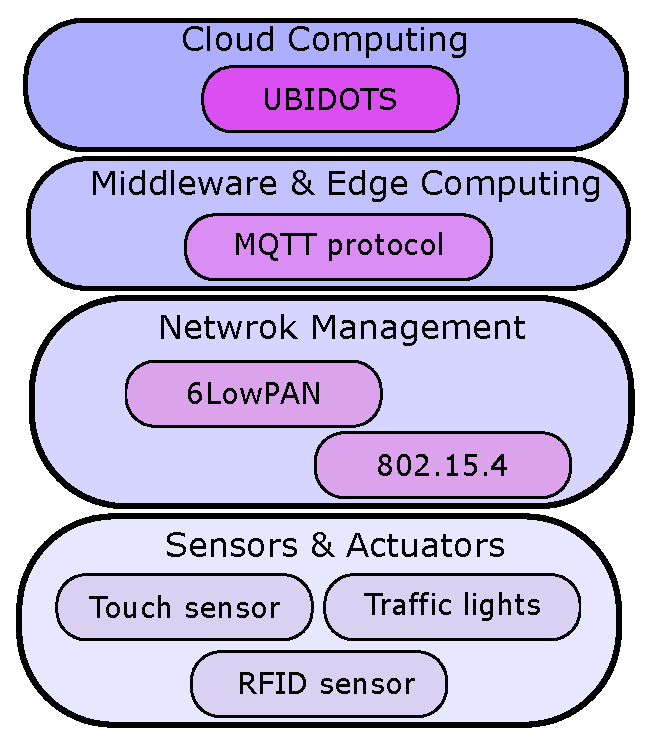
\includegraphics[width=2in]{Figures/StackIoTv1.eps}
\caption{UTLC network layers}
\label{fig:StackIoT.pdf}
\end{figure}

	\section{Discussion} \label{sec:Conclusion}

%purpose
The purpose of the project was to find and examine a communication protocol that could be suitable for IoT applications,
	by investigating the current hardware,
	OS,
	and communication protocols and building a prototype from the selected choices.
What can be said about the investigation is that it is difficult to examine all candidates in detail;
	this means that a rough selection has to be made based on initial knowledge potentially discarding good options.
The general feeling is,
	however,
	that all of the examined candidates in this project were relevant and added valuable insights to the current technology status.
The assessment gave relevant and interesting results that improved the understanding in what IoT can be used for,
	and what further areas of investigation could be.
One of the most interesting areas of further investigation would be the RDC driver,
	as it directly affects the response time and thus also the connection speed.
Even though the power consumption was not in line with the expectations,
	the reason has been found and can be resolved.
Another conclusion is that IoT is not ready for real-time applications as the latency is much higher than expected,
	for the technologies assessed in this thesis,
	and also has a high spread.
As the latency increases for each subsequent network hop and the minimum observed latency per hop is 11ms,
	when using the always-on RDC,
	this type of communication will probably only be used for applications where response time can vary greatly,
	without affecting the functionality.
CoAP as a communication protocol shows a lot of promise when combined with 6LoWPAN and IEEE 802.15.4.
It performs well given its simplicity but has one disadvantage:
	the large overhead which comes from the MAC addressing fields in the IEEE 802.15.4 frame.
If this overhead could be reduced from the current 71\% to only 30%,
	the goodput would double.
A solution would be to use a similar mechanism as BLE where the packet size varies depending on application.
Each node also has computing time left as the MCU is more powerful  than needed for the given application;
	an improvement would be to use a less powerful MCU,
	like the ARM Cortex-M0+,
	to reduce the clock speed as suggested in the discussion.
When looking at the future-proof aspect the later suggestion is probably the better,
	as the clock then could be increased if more computing power is needed.
In the future,
	batteries will hopefully be able to store more energy,
	thus increasing the time between battery changes or reducing the battery size.



\printbibliography
\end{document}

